

\tikzset{every picture/.style={line width=0.75pt}} %set default line width to 0.75pt        

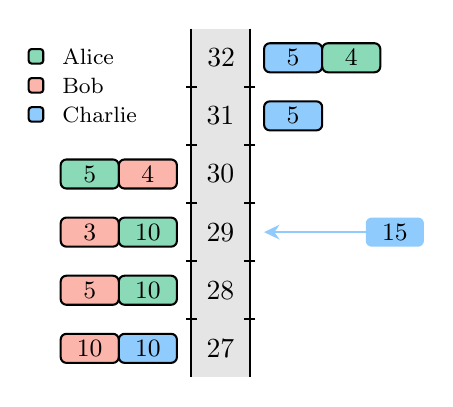
\begin{tikzpicture}[x=0.75pt,y=0.75pt,yscale=-0.7,xscale=0.7]
%uncomment if require: \path (0,300); %set diagram left start at 0, and has height of 300

%Shape: Rectangle [id:dp5750504893681659] 
\draw  [draw opacity=0][fill={rgb, 255:red, 0; green, 0; blue, 0 }  ,fill opacity=0.1 ] (140,30) -- (180,30) -- (180,270) -- (140,270) -- cycle ;
%Rounded Rect [id:dp6877205326451323] 
\draw  [fill={rgb, 255:red, 138; green, 218; blue, 184 }  ,fill opacity=1 ][line width=0.75]  (50,124) .. controls (50,121.79) and (51.79,120) .. (54,120) -- (86,120) .. controls (88.21,120) and (90,121.79) .. (90,124) -- (90,136) .. controls (90,138.21) and (88.21,140) .. (86,140) -- (54,140) .. controls (51.79,140) and (50,138.21) .. (50,136) -- cycle ;
%Straight Lines [id:da215961151995397] 
\draw    (140,30) -- (140,270) (144,70) -- (136,70)(144,110) -- (136,110)(144,150) -- (136,150)(144,190) -- (136,190)(144,230) -- (136,230) ;
%Straight Lines [id:da620143052535216] 
\draw    (180,30) -- (180,270) (184,70) -- (176,70)(184,110) -- (176,110)(184,150) -- (176,150)(184,190) -- (176,190)(184,230) -- (176,230) ;
%Rounded Rect [id:dp9487758453323831] 
\draw  [fill={rgb, 255:red, 251; green, 181; blue, 170 }  ,fill opacity=1 ][line width=0.75]  (50,164) .. controls (50,161.79) and (51.79,160) .. (54,160) -- (86,160) .. controls (88.21,160) and (90,161.79) .. (90,164) -- (90,176) .. controls (90,178.21) and (88.21,180) .. (86,180) -- (54,180) .. controls (51.79,180) and (50,178.21) .. (50,176) -- cycle ;
%Rounded Rect [id:dp2348115833646376] 
\draw  [fill={rgb, 255:red, 138; green, 218; blue, 184 }  ,fill opacity=1 ][line width=0.75]  (90,164) .. controls (90,161.79) and (91.79,160) .. (94,160) -- (126,160) .. controls (128.21,160) and (130,161.79) .. (130,164) -- (130,176) .. controls (130,178.21) and (128.21,180) .. (126,180) -- (94,180) .. controls (91.79,180) and (90,178.21) .. (90,176) -- cycle ;
%Rounded Rect [id:dp2584842224306618] 
\draw  [fill={rgb, 255:red, 138; green, 218; blue, 184 }  ,fill opacity=1 ][line width=0.75]  (90,204) .. controls (90,201.79) and (91.79,200) .. (94,200) -- (126,200) .. controls (128.21,200) and (130,201.79) .. (130,204) -- (130,216) .. controls (130,218.21) and (128.21,220) .. (126,220) -- (94,220) .. controls (91.79,220) and (90,218.21) .. (90,216) -- cycle ;
%Rounded Rect [id:dp05087451015493316] 
\draw  [fill={rgb, 255:red, 251; green, 181; blue, 170 }  ,fill opacity=1 ][line width=0.75]  (50,204) .. controls (50,201.79) and (51.79,200) .. (54,200) -- (86,200) .. controls (88.21,200) and (90,201.79) .. (90,204) -- (90,216) .. controls (90,218.21) and (88.21,220) .. (86,220) -- (54,220) .. controls (51.79,220) and (50,218.21) .. (50,216) -- cycle ;
%Rounded Rect [id:dp9710519793908792] 
\draw  [fill={rgb, 255:red, 251; green, 181; blue, 170 }  ,fill opacity=1 ][line width=0.75]  (50,244) .. controls (50,241.79) and (51.79,240) .. (54,240) -- (86,240) .. controls (88.21,240) and (90,241.79) .. (90,244) -- (90,256) .. controls (90,258.21) and (88.21,260) .. (86,260) -- (54,260) .. controls (51.79,260) and (50,258.21) .. (50,256) -- cycle ;
%Rounded Rect [id:dp7721373725752443] 
\draw  [fill={rgb, 255:red, 138; green, 218; blue, 184 }  ,fill opacity=1 ][line width=0.75]  (28,46) .. controls (28,44.9) and (28.9,44) .. (30,44) -- (36,44) .. controls (37.1,44) and (38,44.9) .. (38,46) -- (38,52) .. controls (38,53.1) and (37.1,54) .. (36,54) -- (30,54) .. controls (28.9,54) and (28,53.1) .. (28,52) -- cycle ;
%Rounded Rect [id:dp4648823353022742] 
\draw  [fill={rgb, 255:red, 143; green, 203; blue, 253 }  ,fill opacity=1 ][line width=0.75]  (28,86) .. controls (28,84.9) and (28.9,84) .. (30,84) -- (36,84) .. controls (37.1,84) and (38,84.9) .. (38,86) -- (38,92) .. controls (38,93.1) and (37.1,94) .. (36,94) -- (30,94) .. controls (28.9,94) and (28,93.1) .. (28,92) -- cycle ;
%Rounded Rect [id:dp396175075326069] 
\draw  [fill={rgb, 255:red, 251; green, 181; blue, 170 }  ,fill opacity=1 ][line width=0.75]  (28,66) .. controls (28,64.9) and (28.9,64) .. (30,64) -- (36,64) .. controls (37.1,64) and (38,64.9) .. (38,66) -- (38,72) .. controls (38,73.1) and (37.1,74) .. (36,74) -- (30,74) .. controls (28.9,74) and (28,73.1) .. (28,72) -- cycle ;
%Rounded Rect [id:dp10932219999579096] 
\draw  [fill={rgb, 255:red, 143; green, 203; blue, 253 }  ,fill opacity=1 ][line width=0.75]  (190,44) .. controls (190,41.79) and (191.79,40) .. (194,40) -- (226,40) .. controls (228.21,40) and (230,41.79) .. (230,44) -- (230,56) .. controls (230,58.21) and (228.21,60) .. (226,60) -- (194,60) .. controls (191.79,60) and (190,58.21) .. (190,56) -- cycle ;
%Rounded Rect [id:dp9836145210038129] 
\draw  [fill={rgb, 255:red, 143; green, 203; blue, 253 }  ,fill opacity=1 ][line width=0.75]  (90,244) .. controls (90,241.79) and (91.79,240) .. (94,240) -- (126,240) .. controls (128.21,240) and (130,241.79) .. (130,244) -- (130,256) .. controls (130,258.21) and (128.21,260) .. (126,260) -- (94,260) .. controls (91.79,260) and (90,258.21) .. (90,256) -- cycle ;
%Rounded Rect [id:dp5732951285894992] 
\draw  [fill={rgb, 255:red, 138; green, 218; blue, 184 }  ,fill opacity=1 ][line width=0.75]  (230,44) .. controls (230,41.79) and (231.79,40) .. (234,40) -- (266,40) .. controls (268.21,40) and (270,41.79) .. (270,44) -- (270,56) .. controls (270,58.21) and (268.21,60) .. (266,60) -- (234,60) .. controls (231.79,60) and (230,58.21) .. (230,56) -- cycle ;
%Straight Lines [id:da15472498021828307] 
\draw [color={rgb, 255:red, 143; green, 203; blue, 253 }  ,draw opacity=1 ]   (260,170) -- (193,170) ;
\draw [shift={(190,170)}, rotate = 360] [fill={rgb, 255:red, 143; green, 203; blue, 253 }  ,fill opacity=1 ][line width=0.08]  [draw opacity=0] (10.72,-5.15) -- (0,0) -- (10.72,5.15) -- (7.12,0) -- cycle    ;
%Rounded Rect [id:dp20817918206073804] 
\draw  [draw opacity=0][fill={rgb, 255:red, 143; green, 203; blue, 253 }  ,fill opacity=1 ][dash pattern={on 4.5pt off 4.5pt}][line width=0.75]  (260,164) .. controls (260,161.79) and (261.79,160) .. (264,160) -- (296,160) .. controls (298.21,160) and (300,161.79) .. (300,164) -- (300,176) .. controls (300,178.21) and (298.21,180) .. (296,180) -- (264,180) .. controls (261.79,180) and (260,178.21) .. (260,176) -- cycle ;
%Rounded Rect [id:dp8342306342416866] 
\draw  [fill={rgb, 255:red, 251; green, 181; blue, 170 }  ,fill opacity=1 ][line width=0.75]  (90,124) .. controls (90,121.79) and (91.79,120) .. (94,120) -- (126,120) .. controls (128.21,120) and (130,121.79) .. (130,124) -- (130,136) .. controls (130,138.21) and (128.21,140) .. (126,140) -- (94,140) .. controls (91.79,140) and (90,138.21) .. (90,136) -- cycle ;
%Rounded Rect [id:dp39224731910080646] 
\draw  [fill={rgb, 255:red, 143; green, 203; blue, 253 }  ,fill opacity=1 ][line width=0.75]  (190,84) .. controls (190,81.79) and (191.79,80) .. (194,80) -- (226,80) .. controls (228.21,80) and (230,81.79) .. (230,84) -- (230,96) .. controls (230,98.21) and (228.21,100) .. (226,100) -- (194,100) .. controls (191.79,100) and (190,98.21) .. (190,96) -- cycle ;

% Text Node
\draw (160,90) node    {$31$};
% Text Node
\draw (160,129.5) node    {$30$};
% Text Node
\draw (70,130) node  [font=\small]  {${\textstyle 5}$};
% Text Node
\draw (160,170) node    {$29$};
% Text Node
\draw (160,210) node    {$28$};
% Text Node
\draw (160,250) node    {$27$};
% Text Node
\draw (70,170) node  [font=\small]  {$3$};
% Text Node
\draw (110,170) node  [font=\small]  {$10$};
% Text Node
\draw (110,210) node  [font=\small]  {$10$};
% Text Node
\draw (70,210) node  [font=\small]  {${\textstyle 5}$};
% Text Node
\draw (70,250) node  [font=\small]  {$10$};
% Text Node
\draw (49,42) node [anchor=north west][inner sep=0.75pt]  [font=\footnotesize] [align=left] {Alice};
% Text Node
\draw (49,62) node [anchor=north west][inner sep=0.75pt]  [font=\footnotesize] [align=left] {Bob};
% Text Node
\draw (49,82) node [anchor=north west][inner sep=0.75pt]  [font=\footnotesize] [align=left] {Charlie};
% Text Node
\draw (160.5,50) node    {$32$};
% Text Node
\draw (210,50) node  [font=\small]  {$5$};
% Text Node
\draw (110,250) node  [font=\small]  {$10$};
% Text Node
\draw (250,50) node  [font=\small]  {$4$};
% Text Node
\draw (280,170) node  [font=\small]  {$15$};
% Text Node
\draw (110,130) node  [font=\small]  {$4$};
% Text Node
\draw (210,90) node  [font=\small]  {$5$};


\end{tikzpicture}
